
%----------------------------------------------------------------------------------------
%	PACKAGES AND OTHER DOCUMENT CONFIGURATIONS
%----------------------------------------------------------------------------------------

\documentclass[twoside, column]{article}
% For two column: \documentclass[twoside, twocolumn]{article}

\usepackage{blindtext} % Package to generate dummy text throughout this template 

\usepackage[sc]{mathpazo} % Use the Palatino font
\usepackage[T1]{fontenc} % Use 8-bit encoding that has 256 glyphs
\linespread{1.05} % Line spacing - Palatino needs more space between lines
\usepackage{microtype} % Slightly tweak font spacing for aesthetics

\usepackage[english]{babel} % Language hyphenation and typographical rules

\usepackage[hmarginratio=1:1,top=32mm,columnsep=20pt]{geometry} % Document margins
\usepackage[hang, small,labelfont=bf,up,textfont=it,up]{caption} % Custom captions under/above floats in tables or figures
\usepackage{booktabs} % Horizontal rules in tables

\usepackage{lettrine} % The lettrine is the first enlarged letter at the beginning of the text

\usepackage{enumitem} % Customized lists
\setlist[itemize]{noitemsep} % Make itemize lists more compact

\usepackage{abstract} % Allows abstract customization
\renewcommand{\abstractnamefont}{\normalfont\bfseries} % Set the "Abstract" text to bold
\renewcommand{\abstracttextfont}{\normalfont\small\itshape} % Set the abstract itself to small italic text

\usepackage{titlesec} % Allows customization of titles
\renewcommand\thesection{\Roman{section}} % Roman numerals for the sections
\renewcommand\thesubsection{\roman{subsection}} % roman numerals for subsections
\titleformat{\section}[block]{\large\scshape\centering}{\thesection.}{1em}{} % Change the look of the section titles
\titleformat{\subsection}[block]{\large}{\thesubsection.}{1em}{} % Change the look of the section titles

\usepackage{fancyhdr} % Headers and footers
\pagestyle{fancy} % All pages have headers and footers
\fancyhead{} % Blank out the default header
\fancyfoot{} % Blank out the default footer
\fancyhead[C]{Multi-digit Prediction with Convolutional Neural Networks $\bullet$ 2016} % Custom header text
\fancyfoot[RO,LE]{\thepage} % Custom footer text

\usepackage{titling} % Customizing the title section

\usepackage{hyperref} % For hyperlinks in the PDF

\usepackage[utf8]{inputenc}
\usepackage{minted}

\usepackage{graphicx}
\graphicspath{ {images/} }


%----------------------------------------------------------------------------------------
%	TITLE SECTION
%----------------------------------------------------------------------------------------

\setlength{\droptitle}{-4\baselineskip} % Move the title up

\pretitle{\begin{center}\Huge\bfseries} % Article title formatting
\posttitle{\end{center}} % Article title closing formatting
\title{Large-scale Identification of Multiple Digits From Real-World Images with Convolutional Neural Networks} 
\author{%
\textsc{Ritchie Ng}\\ 
\normalsize National University of Singapore\\ 
\normalsize \href{mailto:ritchieng@u.nus.edu}{ritchieng@u.nus.edu} 
}
\date{\today} % Leave empty to omit a date
\renewcommand{\maketitlehookd}{%
\begin{abstract}
% Dummy abstract text - replace \blindtext with your abstract text
\noindent \blindtext
\end{abstract}
}

%----------------------------------------------------------------------------------------

\begin{document}

% Print the title
\maketitle

%----------------------------------------------------------------------------------------
%	ARTICLE CONTENTS
%----------------------------------------------------------------------------------------

\section{Introduction}

%------------------------------------------------

\subsection{Overview}
This project explores how convolutional neural networks (ConvNets) can be used to effectively identify a series of digits from real-world images that are obtained from \textit{The Street View House Numbers (SVHN) Dataset}.  ConvNets have evolved dramatically every year since the inception of the ImageNet Challenge in 2010. 

A proverbial ConvNet structure is the \textit{LeNet-5} that has relatively few layers of convolutions, poolings, and full connections. Subsequently, with the advent of the ImageNet Challenge, we are experiencing a gradual trend towards deeper ConvNets with more layers and higher accuracy such as \textit{AlexNet}, \textit{ZFNet}, \textit{VGGNet}, \textit{GoogLeNet}, and \textit{ResNet} being the latest state-of-the-art implementation of ConvNets.  

To this point, I started off with a simple ConvNet structure as a base where I made refinements to determine my optimal model for identifying multiple digits from real-world images.

%------------------------------------------------

\subsection{Problem Statement}
I am attempting to predict a series of numbers given an image of house numbers from the SVHN dataset. An important thing to take note is that instead of the standard identification of numbers, as with the MNIST dataset, I now need to correctly detect the numbers and the sequence of numbers. 

%------------------------------------------------

\subsection{Metric}

Across the models, I compared the training, validation and test accuracies. And accuracy is measured by Equation (1).

\begin{equation} \label{}
\frac{TP + TN}{TP + TN + FP + FN}
\end{equation}

Using Numpy, I created an accuracy function that is catered towards the problem of multi-digit prediction. 

\definecolor{bg}{rgb}{0.95,0.95,0.95}
\begin{minted}[bgcolor=bg]{python}
def accuracy(predictions, labels):
    return (100.0 * np.sum(np.argmax(predictions, 2).T == labels)
            / predictions.shape[1] / predictions.shape[0])      
 \end{minted}
 
%------------------------------------------------

\section{Analysis}

%------------------------------------------------
\subsection{Data Exploration}

There are 10 classes in the data, 1 for each digit and 10 denotes '0'. In total, there are 73257 digits for training, 26032 digits for testing, and 531131 extra digits. For my implementation, I used the raw images that came with a variety of dimensions as shown in Figure 1.

\begin{figure}[h]
\caption{Examples of the the database of raw images from SVHN}
\centering
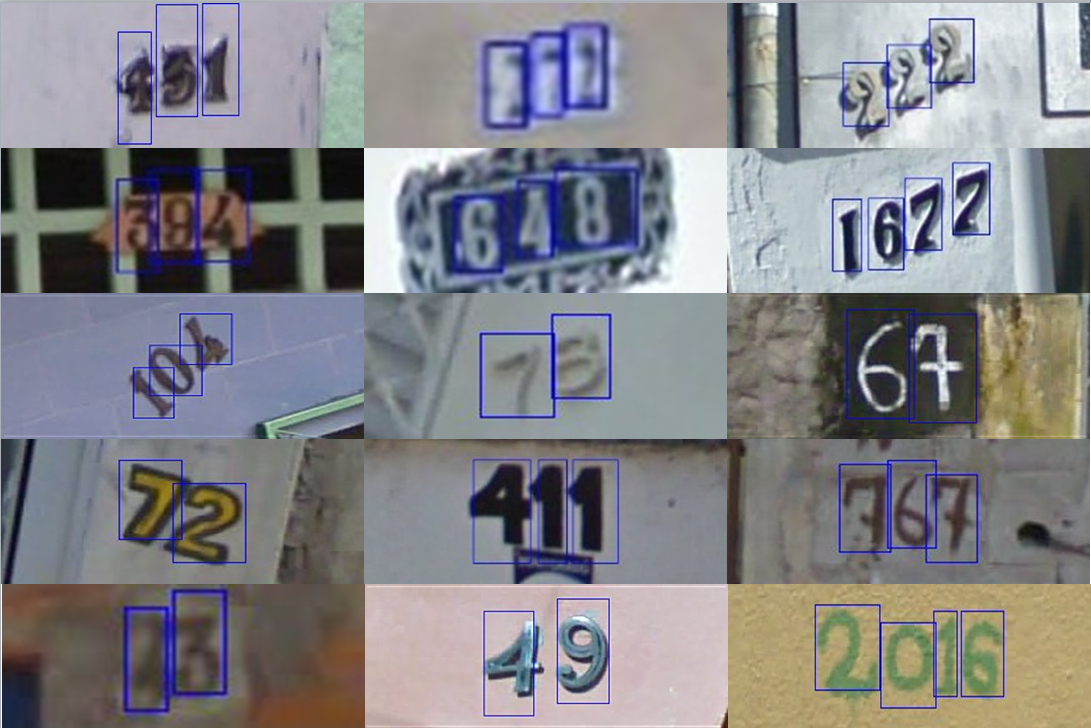
\includegraphics[width=0.5\textwidth]{original_photos}
\end{figure}

\subsection{Exploratory Visualization}

We go into the raw data to further explore the images. 
Text requiring further explanation\footnote{Example footnote}.

%------------------------------------------------

\section{Results}

\begin{table}
\caption{Example table}
\centering
\begin{tabular}{llr}
\toprule
\multicolumn{2}{c}{Name} \\
\cmidrule(r){1-2}
First name & Last Name & Grade \\
\midrule
John & Doe & $7.5$ \\
Richard & Miles & $2$ \\
\bottomrule
\end{tabular}
\end{table}

\blindtext % Dummy text

\begin{equation}
\label{eq:emc}
e = mc^2
\end{equation}

\blindtext % Dummy text

Maecenas sed ultricies felis. Sed imperdiet dictum arcu a egestas. 
\begin{itemize}
\item Donec dolor arcu, rutrum id molestie in, viverra sed diam
\item Curabitur feugiat
\item turpis sed auctor facilisis
\item arcu eros accumsan lorem, at posuere mi diam sit amet tortor
\item Fusce fermentum, mi sit amet euismod rutrum
\item sem lorem molestie diam, iaculis aliquet sapien tortor non nisi
\item Pellentesque bibendum pretium aliquet
\end{itemize}
\blindtext % Dummy text

%------------------------------------------------

\section{Discussion}

\subsection{Subsection One}

A statement requiring citation \cite{Figueredo:2009dg}.
\blindtext % Dummy text

\subsection{Subsection Two}

\blindtext % Dummy text

%----------------------------------------------------------------------------------------
%	REFERENCE LIST
%----------------------------------------------------------------------------------------

\begin{thebibliography}{99} % Bibliography - this is intentionally simple in this template

\bibitem[Figueredo and Wolf, 2009]{Figueredo:2009dg}
Figueredo, A.~J. and Wolf, P. S.~A. (2009).
\newblock Assortative pairing and life history strategy - a cross-cultural
  study.
\newblock {\em Human Nature}, 20:317--330.
 
\end{thebibliography}

%----------------------------------------------------------------------------------------

\end{document}
